\begin{enunciado}
 Se lanza una moneda hasta que sale una cara y se registra el n\'umero
 de lanzamientos $X$.
 Despu\'es de repetir el experimento $256$ veces,
 obtenemos los siguientes resultados:
 \begin{center}
  \begin{tabular}{c|cccccccc}
   $x$ &  $1$  &  $2$ &  $3$ &  $4$ & $5$ & $6$ & $7$ & $8$ \\
   $f$ & $136$ & $60$ & $34$ & $12$ & $9$ & $1$ & $3$ & $1$
  \end{tabular}
 \end{center}
 Con un nivel de significancia de $0.05$ pruebe la hip\'otesis
 de que la distribuci\'on observada de $X$ se puede ajustar
 por la distribuci\'on geom\'etrica $g(x;1/2)$, $x = 1,2,3,\ldots$
\end{enunciado}

\begin{solucion}
 \begin{datos}
  $\phantom{0}$
  \begin{itemize}
   \item Tama\~no de la muestra: $n=256$.
   \item Frecuencias observadas:
   $O = \{o_1=136, o_2=60, o_3=34, o_4=12, o_5=9, o_6=1, o_7=3, o_8=1\}$.
   \item Probabilidades esperadas: como distribuci\'on geom\'etrica
   est\'a definida para cada $x\in\mathbb{N}$, entones $p_i = g(i;1/2) =
   \frac{1}{2} \cdot \left( \frac{1}{2} \right)^{i-1} = 
   \left( \frac{1}{2} \right)^{i} = \frac{1}{2^i}$,
   para cada $i \in \mathbb{N}\cap[1,7]$
   y $p_8 = g(x\geq 8; 1/2) = 1 - \sum_{i=1}^{7} g(i;1/2)
   = 1 - \sum_{i=1}^{7} p_i$.
   Entonces $p_1 = \frac{1}{2}$, $p_2 = \frac{1}{4}$, $p_3 = \frac{1}{8}$,
   $p_4 = \frac{1}{16}$, $p_5 = \frac{1}{32}$, $p_6 = \frac{1}{64}$,
   $p_7 = \frac{1}{128}$
   y, como $\sum_{i=1}^7 p_i=\frac{64+32+16+8+4+2+1}{128}=\frac{127}{128}$, entonces $p_8 = 1 - \frac{127}{128} = \frac{1}{128}$.
   \item Frecuencias esperadas: $E = \left\{
   \left.e_i=n\cdot p_i\,\right|\,\forall i\in\mathbb{N} \right\}
   = \{e_1=128, e_2=64, e_3=32, e_4=16, e_5=8, e_6=4, e_7=2, e_8=2\}$.
  \end{itemize}
  Dado que las pruebas de bondad por m\'etodo de $\chi^2$ no son confiables
  cuando la frecuencia esperada de una celda es menor a $5$,
  se agrupar\'an los datos, como sigue:
  \begin{itemize}
   \item Probabilidades esperadas:
   $\{ p_1 = \frac{1}{2}, p_2 = \frac{1}{4}, p_3 = \frac{1}{8},
   p_4 = \frac{1}{16}, p_5 = \frac{1}{32}, p_6 = \frac{1}{32} \}$.
   \item Frecuencias esperadas:
   $E=\{e_1 = 128, e_2 = 64, e_3 = 32, e_4 = 16, e_5 = 8, e_6 = 8\}$.
   \item Frecuencias observadas:
   $O = \{o_1=136, o_2=60, o_3=34, o_4=12, o_5=9, o_6=5\}$.
   \item Celdas totales del experimento: $k=6$.
   \item Grados de libertad de la prueba $\chi^2$: $v= k-1 = 5$.
  \end{itemize}
 \end{datos}

 \begin{hipotesis}
  Prueba de bondad de ajuste para probar $H_0:$
  que la variable aleatoria $X$, del n\'umero veces
  que se lanz\'o la moneda del enunciado hasta obtener la primera cara,
  sigue una distribuci\'on geom\'etrica
  con par\'ametro $p=\frac{1}{2}$,
  contra la alternativa $H_1$ de que no es as\'{\i}.
 \end{hipotesis}

 \begin{significancia}
  $\alpha = 0.05$.
 \end{significancia}

 \begin{region}
  De la tabla A.5 se tiene el valor cr\'{\i}tico
  $\chi^2_{\alpha,v} = \chi^2_{0.05,5} \approx 11.07$,
  por lo que la regi\'on de rechazo est\'a dado
  para $\chi^2 > 11.07$, donde
  $\chi^2 = \sum_{i=1}^{k} \frac{\left( o_i - e_i \right)^2}{e_i}$.
 \end{region}

 \begin{estadistico}
  \begin{eqnarray*}
   \chi^2 & = & \sum_{i=1}^{k} \frac{\left( o_i - e_i \right)^2}{e_i} \\
   & = & \frac{(136-128)^2}{128} + \frac{(60-64)^2}{64} +
   \frac{(34-32)^2}{32} + \frac{(12-16)^2}{16} +
   \frac{(9-8)^2}{8} + \frac{(5-8)^2}{8} \\
   & = &
   \frac{8^2 + 4^2(2) + 2^2(4) + 4^2(8) + 1^2(16) + 3^2(16)}{128}\\
   & = & \frac{64 + 32 + 16 + 128 + 16 + 144}{128} = \frac{400}{128} \\
   & = & \frac{25}{8} = 3.125
  \end{eqnarray*}
 \end{estadistico}

 \begin{decision}
  No se rechaza $H_0$.
 \end{decision}

 \begin{conclusion}
  No hay evidencia suficiente para rechazar que el experimento
  de lanzar un moneda hasta obtener una cara con la moneda del enunciado
  sea una distribuci\'on distinta de la geom\'etrica
  con par\'ametro $p=\frac{1}{2}$;
  es decir, no se confirma que el experimento no es significativamente
  distinto de esta distribuci\'on.
 \end{conclusion}

 Finalmente, usando el archivo anexo
 \texttt{P15\_Prueba\_de\_bondad\_chi2\_01.r},
 que a su vez requiere los datos del archivo
 \texttt{DB21\_Problema\_085.csv}, con los siguientes cambios:
 \begin{verbatim}
> datos<-read.csv("DB21_Problema_085.csv",sep=";",encoding="UTF-8")
> varInteres<-"Frecuencia"
> varCelda<-"Lanzamientos.cantidad"
> distribucion<-4
> parametro_nombre<-c("p")
> parametro_valor<-c(1/2)
> combinar<-TRUE
> grafica<-TRUE
> tituloEjeX<-"Primera aparición de cara en los lanzamientos de una moneda"
> alfa<-0.05
 \end{verbatim}
 \vspace{-0.7cm}
 el programa de R lanza el siguiente resultado:
 \begin{verbatim}
               Variable Distribución de ajuste   p Estadístico Chisq2
1 Lanzamientos.cantidad             Geométrica 0.5              3.125
  Grados de libertad   Valor-p alpha Región de Rechazo
1                  5 0.6807215  0.05      > 11.0704977
                          Resultado
1 No se rechaza el ajuste de bondad
 \end{verbatim}
 \vspace{-0.7cm}
 que incluye la siguiente figura:
 \begin{center}
  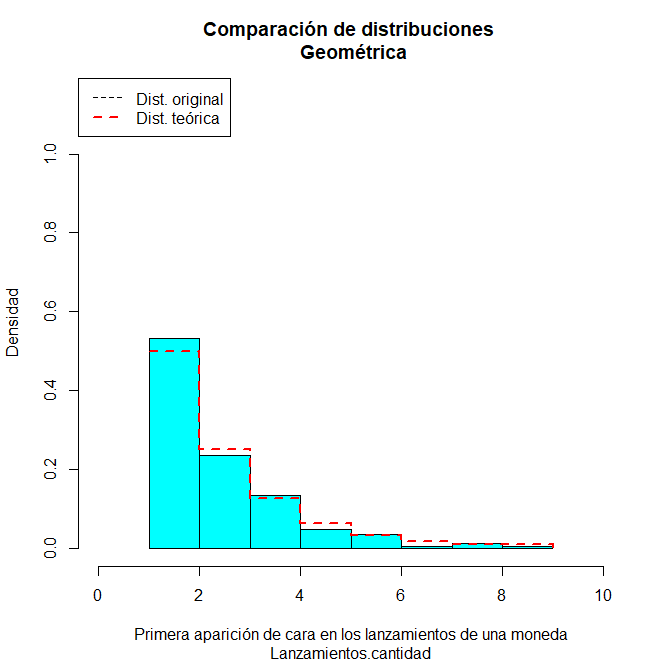
\includegraphics[scale=0.35]{Problema_85.png}
 \end{center}
 El cual coincide con los datos obtenidos,
 que es a lo que se quer\'{\i}a llegar.${}_{\blacksquare}$
\end{solucion}
